\chapter{Quasi-Toeplitz Configurations}\label{chapter:Toeplitz}

In this chapter we develop tools necessary in our approach of proving Theorem~\ref{Krieger2}. More specifically, we recall the notion of a Toeplitz sequence (see \cite{JK69}, \cite{DI88})
and its generalization\footnote{Toeplitz sequence is a two-sided sequence, hence a function defined over $\Z$, such that its every element occurs periodically. Its first generalization is a Toeplitz configuration, which is defined over an amenable residually finite group $G$ instead of $\Z$. Toeplitz configurations were widely studied in \cite{CP14}, \cite{CP08}, \cite{Krieger10}.}: a quasi-Toeplitz configuration (see \cite{CC19}) and study their properties. Most importantly, we show that the orbit closure of a quasi-Toeplitz configuration forms a minimal subsystem (see also \cite{CC19}), and further that the set of all quasi-Toeplitz configurations is path-connected with respect to the Weyl pseudometric (defined in Section~\ref{section:weyl}). 
These are the two main observations that allow us later to derive Theorem~\ref{Krieger2}.

\section{Definition}
In this chapter we assume that $G$ is a congruent monotileable, hence amenable, group. We work with the shift space $\alf^G$ where $\alf$ is a finite alphabet. What follows is a definition of a quasi-Toeplitz configuration.
\begin{defn}[Quasi-Toeplitz Configuration]\label{def:toeplitz}
An element $x\in \alf^G$ is called a {\bf quasi-Toeplitz configuration} if there exists a congruent \Folner sequence $\{F_n\}_{n\in\N}$ with an associated \elegant sequence of centers $\{C_n\}_{n\in\N}$ (see Lemma \ref{lem:elegant_C_n}) such that for every $g\in G$ there exists $m\in\N$ such that $ x(g)= x(gc)$ for any $c\in C_m$.
\end{defn}
\noindent
It is also convenient to introduce the following notation: given $C\subseteq G$ and $x\in\alf^G$ we define
\begin{align*}
\text{Per}_{C}(x)&\defeq\big\{g\in G\,:\, x(g)=x(gh )\text{ for every }h\in C\big\}.
 \end{align*}
With this notation it is not hard to see that $x\in  \alf^G$ is a quasi-Toeplitz configuration if and only if there exists a congruent \Folner  sequence $\{F_n\}_{n\in\N}$ with an \elegant sequence of centers $\{C_n\}_{n\in\N}$ satisfying
\[
\bigcup_{n=0}^{\infty}\Per_{C_n}(x)=G.
\]
Quasi-periodic configuration is a special case of quasi-Toeplitz configurations.
\begin{defn}[Quasi-periodic configuration]
An element $x\in \alf^G$ is a {\bf quasi-periodic configuration} if there exists a congruent \Folner sequence $\{F_n\}_{n\in\N}$ with an \elegant sequence of centers $\{C_n\}_{n\in\N}$ and there exists $N\in\N$ such that for every $g\in G$ it holds $ x(g)= x(gc)$ for any $c\in C_N$. Then we say that $x$ is quasi-periodic with period $C_N$.
\end{defn}


\section{Examples}
Before we proceed with the study of properties of quasi-Toeplitz configurations we give some examples to provide intuitions and help in visualizing this important notion.
%
We discuss two special cases: when $G=\Z$ and when $G=\Q$. 
\subsection{Toeplitz Sequences over $\Z$}
In the case of $G=\Z$, quasi-Toeplitz configurations coincide with the notion of Toeplitz sequences and are well studied in the literature \cite{JK69}, \cite{DI88}, \cite{AKL16}, \cite{Downarowicz05}.
%
In fact, the definition of quasi-Toeplitz configurations comes as a generalization of Toeplitz sequences from $\Z$ to more general groups.
%
For clarity we repeat the definition for this special case.
\begin{defn}[Toeplitz Sequence]
We call $x\in\alf^{\Z}$ a Toeplitz seqence if each of its elements occurs periodically, i.e., for every $n\in\Z$ there exists $p\in\N$ such that we have $x(n+ip)=x(n)$  for every $i\in\Z$.
\end{defn}

\begin{rem}
Notice that if $x\in\alf^Z$ satisfies the above definition then it also satisfies Definition~\ref{def:toeplitz} in case $G=\Z$. Indeed, let $F_n=\{0,1,\ldots,n!-1\}$ and $C_n=n!\Z$ for every $n\in\N$. If $x(n)\in\alf$ (for some $n\in\N$) occurs with some period $p\in\N$, then $x(n)=x(n+c)$ for every $c\in C_p$.
\end{rem}
\noindent 
We now proceed  with a construction of Toeplitz sequences that is in a sense ``complete'', i.e., each sequence constructed this way is Toeplitz, and also each Toeplitz sequence can be constructed this way (by an appropriate choice of parameters of the construction).

\subsubsection{Construction of a Toeplitz sequence over $\Z$.}
We construct Toeplitz sequences inductively. For this, it is convenient to temporarily ``add'' to the alphabet $\alf$ a symbol ``$\star$'' denoting ``empty place'' and obtain a new alphabet $\alf_{\star}=\alf\cup\{\star\}$.  

\noindent {\bf Base step.} We start with a sequence of ``empty places'' $x_0\in\alf_{\star}^{\Z}$ satisfying $x_0\equiv \star$.
%
Now, the idea is to ``exhaust'' all the empty places one by one.

\noindent {\bf Induction step.} In the $n$-th step (with $n\geq 1$) we construct $x_n\in\alf_{\star}^{\Z}$ as follows: if there is no star left in $x_{n-1}$ then we end the construction by setting $x_n=x_{n+1}=x_{n+2}=\ldots = x_{n-1}$.
 %
Otherwise we pick an index $k_n\in \Z$ to be the $k$ such that $x_{n-1}(k)=\star$ and $k$ has the smallest absolute value out of all such (with ties resolved arbitrarily).
%

Next, we choose an element $a_n \in \alf$ and assign it to position $k_n$.
%
Finally, we need to decide on the period $p_n \in \N$ that determines how often the newly assigned element will repeat.
% 
Note that $p_n$ needs to satisfy the condition that all the positions among $k_n + p_n \Z$ are occupied by $\star$'s in $x_{n-1}$, otherwise we would override some previously set value.
%
It is not hard to see that indeed such a period always exists. 
%
At the end, we  modify $x_{n-1}$ by ``filling empty places'' with $a_n$ at appropriate positions to obtain $x_n$, thus formally
\[
x_n(k)=\begin{cases}
a_n &\text{ if } k\in k_n+p_n\Z,\\
x_{n-1}(k) & \text{ otherwise}.
\end{cases}
\]
\noindent {\bf Limit step.}
Having $\{x_n\}_{n\in\N}$ constructed, we set
\[x=\lim_{n\to\infty}x_n.\]
\noindent We refer to Figure~\ref{fig:toeplitz-z} for an example of how such a construction might look like. %\todo{fix the figure.}
\begin{figure}
\[
 \begin{array}{ *{18}{l} }
 & x_0\colon &\ldots& \star & \star & \star & \star & \star & \star & .\star & \star & \star &\star & \star & \star & \star & \star&\ldots \\
 %
p_1=3, &x_1\colon&\ldots& \bm{a_1} & \star & \star & \bm{a_1} & \star & \star &.\bm{a_1} & \star & \star & \bm{a_1}  & \star &\star & \bm{a_1} & \star &\ldots \\
%
p_2=6,&x_2\colon &\ldots&a_1 &\bm{a_2} & \star & a_1 & \star & \star & .a_1 &\bm{a_2} & \star &a_1 & \star & \star & a_1 &\bm{a_2}&\ldots \\
%
p_3=6, &x_3\colon &\ldots&a_1 & a_2 & \star & a_1 & \star & \bm{a_3} & .a_1 & a_2 & \star & a_1 & \star & \bm{a_3} &a_1 & a_2&\ldots \\
%
p_4=12, &x_4\colon&\ldots&a_1 & a_2 & \star & a_1 & \star & {a_3} & .a_1 & a_2 & \bm{a_4}& a_1 & \star & {a_3} &a_1 & a_2&\ldots \\
%
p_5=6, &x_5\colon &\ldots&a_1 & a_2 & \star & a_1 & \bm{a_5} & {a_3} & .a_1 & a_2 & {a_4} & a_1 &\bm{a_5} & {a_3} &a_1 & a_2&\ldots \\
 \end{array}
\]
\caption{An example of a construction of a Toeplitz sequence over $\Z$.}\label{fig:toeplitz-z}
\end{figure}

\subsection{Quasi-Toeplitz Configurations over $\Q$}
The second example we would like to demonstrate is when $G=(\Q, +)$ (for simplicity we also choose $\alf = \{0,1\}$).  
%
We note that this case is fundamentally different to $\Z$, as the additive group of rationals is not  residually finite (since it is abelian and not finitely generated).
%
Still, $\Q$ is congruent monotileable, which, as it turns out, is enough to prove interesting properties of quasi-Toeplitz configurations in this setting. 


We would like to assign $0$'s and $1$'s to rational numbers such that they appear with some ``period'' given by a set of centers associated with a certain monotile.
%
Therefore we first need to construct a congruent \Folner sequence. 
%
Before we proceed with the construction, we introduce some useful notation.  
In this section we  denote intervals of rational numbers by $(a,b)$, instead of $(a,b) \cap \Q$. 
We start with a definition of a set that serves as a fundamental building block for creating monotiles
\[
J(a,b,k)\defeq [a,b)\cap\inbrace{\frac{j}{k}:j\in\Z }\quad \text{ for } a,b\in\Z~~k\in\N\setminus\{0\}.
\]
Notice that $J(a,b,k)$ is a monotile since 
\begin{equation*}\label{eq:defCabk}
C(a,b,k)\defeq\left[0,\frac{1}{k}\right)+(b-a)\Z
\end{equation*}
is the set of centers associated with $J(a,b,k)$. We define the following two operations on $J(a,b,k)$ (see also Figure~\ref{fig:folner_in_Q} for a graphical explanation):
\begin{enumerate}
\item $\ext \insquare{J(a,b,k)}\defeq (J(a,b,k)-(b-a))\sqcup J(a,b,k)\sqcup (J(a,b,k)+(b-a)) $,
\item  $\displaystyle \cond \insquare{J(a,b,k),p}\defeq \bigsqcup_{j=0}^{p-1}\inparen{J(a,b,k)+\frac{j}{kp}}, ~~$ for any positive integer $p$.
\end{enumerate}
%
Observe that the operation $\ext$ triples the length of $J(a,b,k)$ by attaching both to the left and to the right of it a shifted copy of it. The $\cond$ operation makes $p$ copies of the set $J(a,b,k)$ and puts them one after another with spacing $\frac{1}{kp}$.
%
Moreover, the following relations hold
\begin{align*}
&\ext \insquare{ J(a,b,k)} = J(a-(b-a), b+(b-a),k), \\
&\cond \insquare{ J(a,b,k),p}=J(a,b,kp).
\end{align*}
%
Note that both these operations given a monotile create a new monotile by copying and shifting a certain number of copies of the initial monotile.
% 
It is therefore not a surprise that we can use these operations to construct a congruent \Folner sequence $\F=\{F_n\}_{n\in\N}$.
%
Essentially, the only non-trivial constraint to satisfy is that $\bigcup\F=\Q$.
%
Towards this end, we need to keep extending our monotile and carefully use the condense operation.
%
For this purpose define a sequence of primes $\{q_i\}_{i\in\N}\subseteq\N$  such that every prime number occurs infinitely many times, that is,  for every $p\in\mbP$ the set $\inbrace{i:q_i=p}$ is infinite (where $\mbP$ denotes the set of primes). 

Now we are ready to construct $\F=\{F_n\}_{n\in\N}$. The construction is inductive. 
%
In the base step $n=0$ we put $F_0\defeq J(0,1,1)$, that is, $F_0=\{0\}.$ 
%
Next assume that we have already constructed $F_n$ for some $n\in\N$. 
%
We define $F_{n+1}$ as follows (see Figure \ref{fig:folner_in_Q})
\begin{align*}
&F_{n+1}'\defeq \ext \insquare{F_n}, \\
&F_{n+1} \defeq \cond \insquare{ F_{n+1}', q_{n}}.
\end{align*}

\begin{figure}
\centering
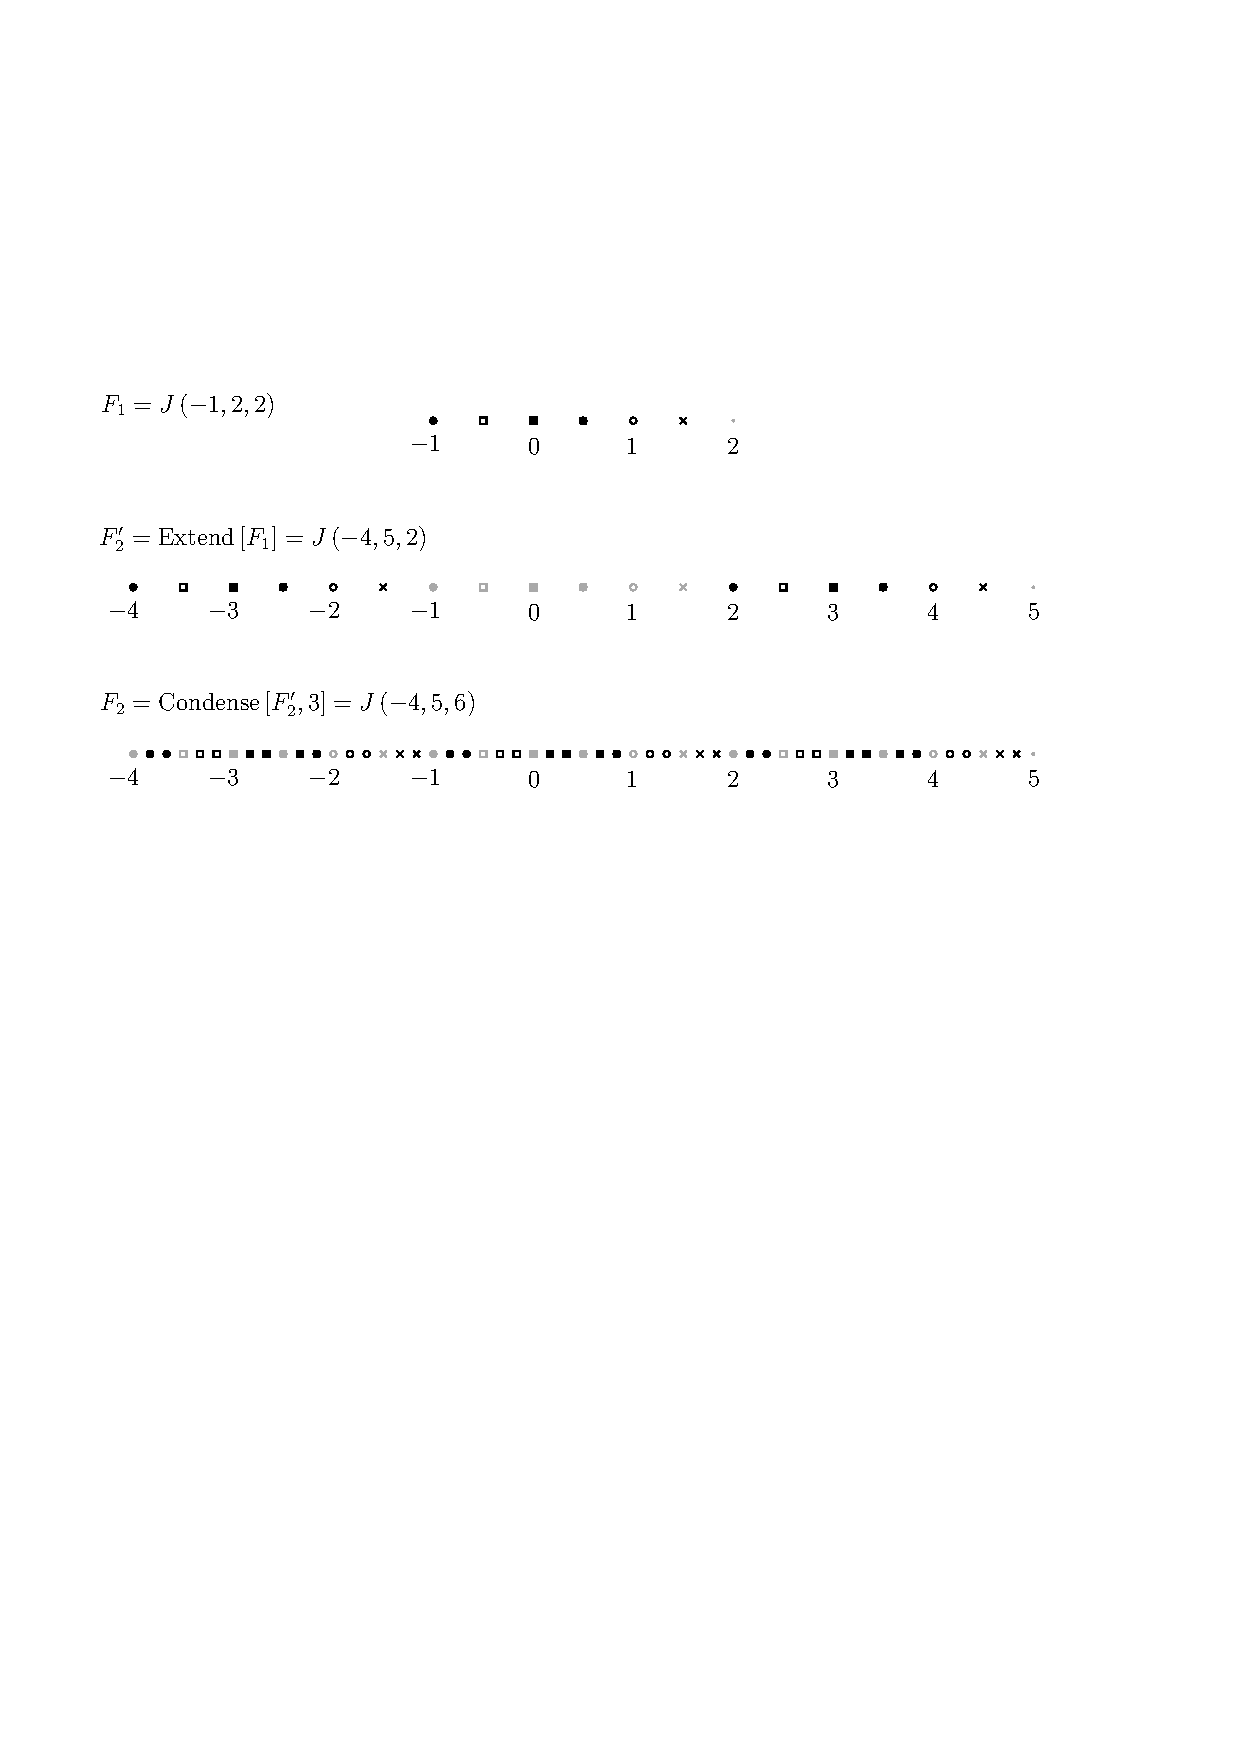
\includegraphics[scale=0.9]{Graphics/folnerQ}
\caption{An illustration of the second step of the construction of a congruent \Folner seqence $\F=\{F_n\}_{n\in\N}$ in $(\Q,+)$ with $\{q_i\}_{i\in\N}$ such that $q_0=2$ and $q_1=3$. We start with $F_1$ already constructed. Its elements are marked with different symbols to better illustrate how does $F_2$ arise by copying and shifting $F_1$. New copies obtained as a result of the  $\ext$ and $\cond$ operations respectively are marked with black, and their arguments are grey.}\label{fig:folner_in_Q}
\end{figure}

We now justify that such a sequence $\F$ indeed satisfies $\bigcup\F=\Q$.
%
Let $p,q\in\Z$. We show that there exists $N\in\N$ such that $\frac{p}{q}\in F_N$. For $n\in\N$ define $\alpha_n, a_n, b_n$ such that
\[
F_n = J(a_n, b_n, \alpha_n).
\]
It is not hard to verify by induction that $a_n=-\frac{1}{2}(3^n-1)$, $b_n=\frac{1}{2}(3^n+1)$ and $\alpha_n = \prod_{i=0}^{n-1} q_i$. 
Since, $\{q_i\}_{i\in\N}$ contains every prime infinitely many times, there exists $n_1\in\N$ such that $q$ divides $\alpha_{n_1}$.
We can also find $n_2\in \N$ satisfying 
\[
a_{n_2} < \frac{p}{q} <b_{n_2},
\]
since clearly $a_n \to -\infty$ and $b_n \to \infty$.
%
By taking $N\defeq\max\{n_1,n_2\}$ we obtain that, by definition, $\frac{p}{q} \in F_N$.

It is easy to see from the construction of $\F$ that remaining conditions from Definition \ref{def:congruent_monotilable} and the \Folner condition are satisfied.
Therefore $\{F_n\}_{n\in\N}$ is a congruent \Folner sequence.

\bigskip
Now we construct a quasi-Toeplitz configuration $x\in\{0,1\}^{\Q}$ with respect to the congruent \Folner sequence $\F$ in a similar way to how we built a Toeplitz sequence in $\{0,1\}^{\Z}$. Fix an arbitrary enumeration of elements of $\Q$. Denote by $\{C_n\}_{n\in\N}$ the sequence of centers associated with the sets in $\F$. 

In the base step $n=0$ we arbitrarily define $x(g)$ for $g$ in some arbitrarily chosen set $G_0\subseteq F_{0}$ (in particular, we might choose $G_0 = \emptyset$). Then copy this ``pattern to the set $G_0+C_0\subseteq\Q$, that is, put $x(g+h)\defeq x(g)$ for $g\in G_0$ and $h\in C_{0}$. Therefore in the base step we define $x$ on the set $G_0+C_{0}$, i.e., set $x(g+c)=x(g)$ for all $g\in G_0$ and $c\in C_0$. 
%
At the start of the $(n+1)$-th step of the construction we have $x$ defined on the set of indices
\[
T_n\defeq \bigsqcup_{i=0}^n (G_i+C_i).
\]
We simply choose a new set $G_{n+1}\subseteq F_{n+1}\setminus T_n$ such that in the first place we choose available elements from $F_{n+1}$ with the smallest index (according to the enumeration of $\Q$). Next we define $x$ on $G_{n+1}$ and extend this ``pattern'' to the set $G_{n+1}+C_{n+1}$, that is, we set $x(g+h)\defeq x(g)$ for $g\in G_{n+1}$ and $h\in C_{n+1}$.

Note that choosing $T_n$ according to the enumeration of $\Q$  for every $n\in\N$, guarantees that $\bigcup_{n\in\N}T_n=\Q$, thus $x$ is defined over all elements in $\Q$.

As an example, we show two steps of the above construction with $\F$ defined for $\{q_i\}_{i\in\N}$ satisfying $q_0=2$ and $q_1=3$ (see Figure \ref{fig:toeplitzQ}). For $F_1$ and $F_2$ in this setting, see Figure \ref{fig:folner_in_Q}. Choose $G_0\defeq \emptyset$.
%
Subsequently, we let $G_1\defeq\inbrace{-1, 0, \frac{1}{2},1 }$. We define $x$ on $G_1$ and extend this to $G_1+C_1$ (for the formula for $C_1$ see \eqref{eq:defCabk})
\[
x(r)\defeq \begin{cases}1 & \text{if } r\in\inbrace{-1, 0, \frac{1}{2}}+\left[0,\frac{1}{2}\right) + 3\Z, \\ 0  & \text{if } r\in 1+\left[0,\frac{1}{2}\right)+3\Z. \end{cases}
\]
Next, we define $G_2\subseteq F_2$. We work here with an enumeration of elements in $G$ that is consistent with $\F$ and thus we choose to $G_2$ elements from $F_1\setminus G_1$, we set $G_2\defeq\inbrace{-3\frac{2}{6},-\frac{1}{2}, -\frac{1}{6}, 1\frac{1}{2}, 1\frac{4}{6}, 4\frac{4}{6}, 4\frac{5}{6} }$. Then we define $x$ on $G_2$ and extend it to $G_2 +C_2$ as follows
\[
x(r)\defeq \begin{cases}1 & \text{if } r\in\inbrace{1\frac{1}{2}, 1\frac{4}{6}}+\left[0,\frac{1}{6}\right) + 9\Z, \\ 0  & \text{if } r\in\inbrace{-3\frac{2}{6}, -\frac{1}{2},-\frac{1}{6},4\frac{4}{6}, 4\frac{5}{6}}+\left[0,\frac{1}{6}\right)+9\Z. \end{cases}
\]

\begin{figure}
\centering
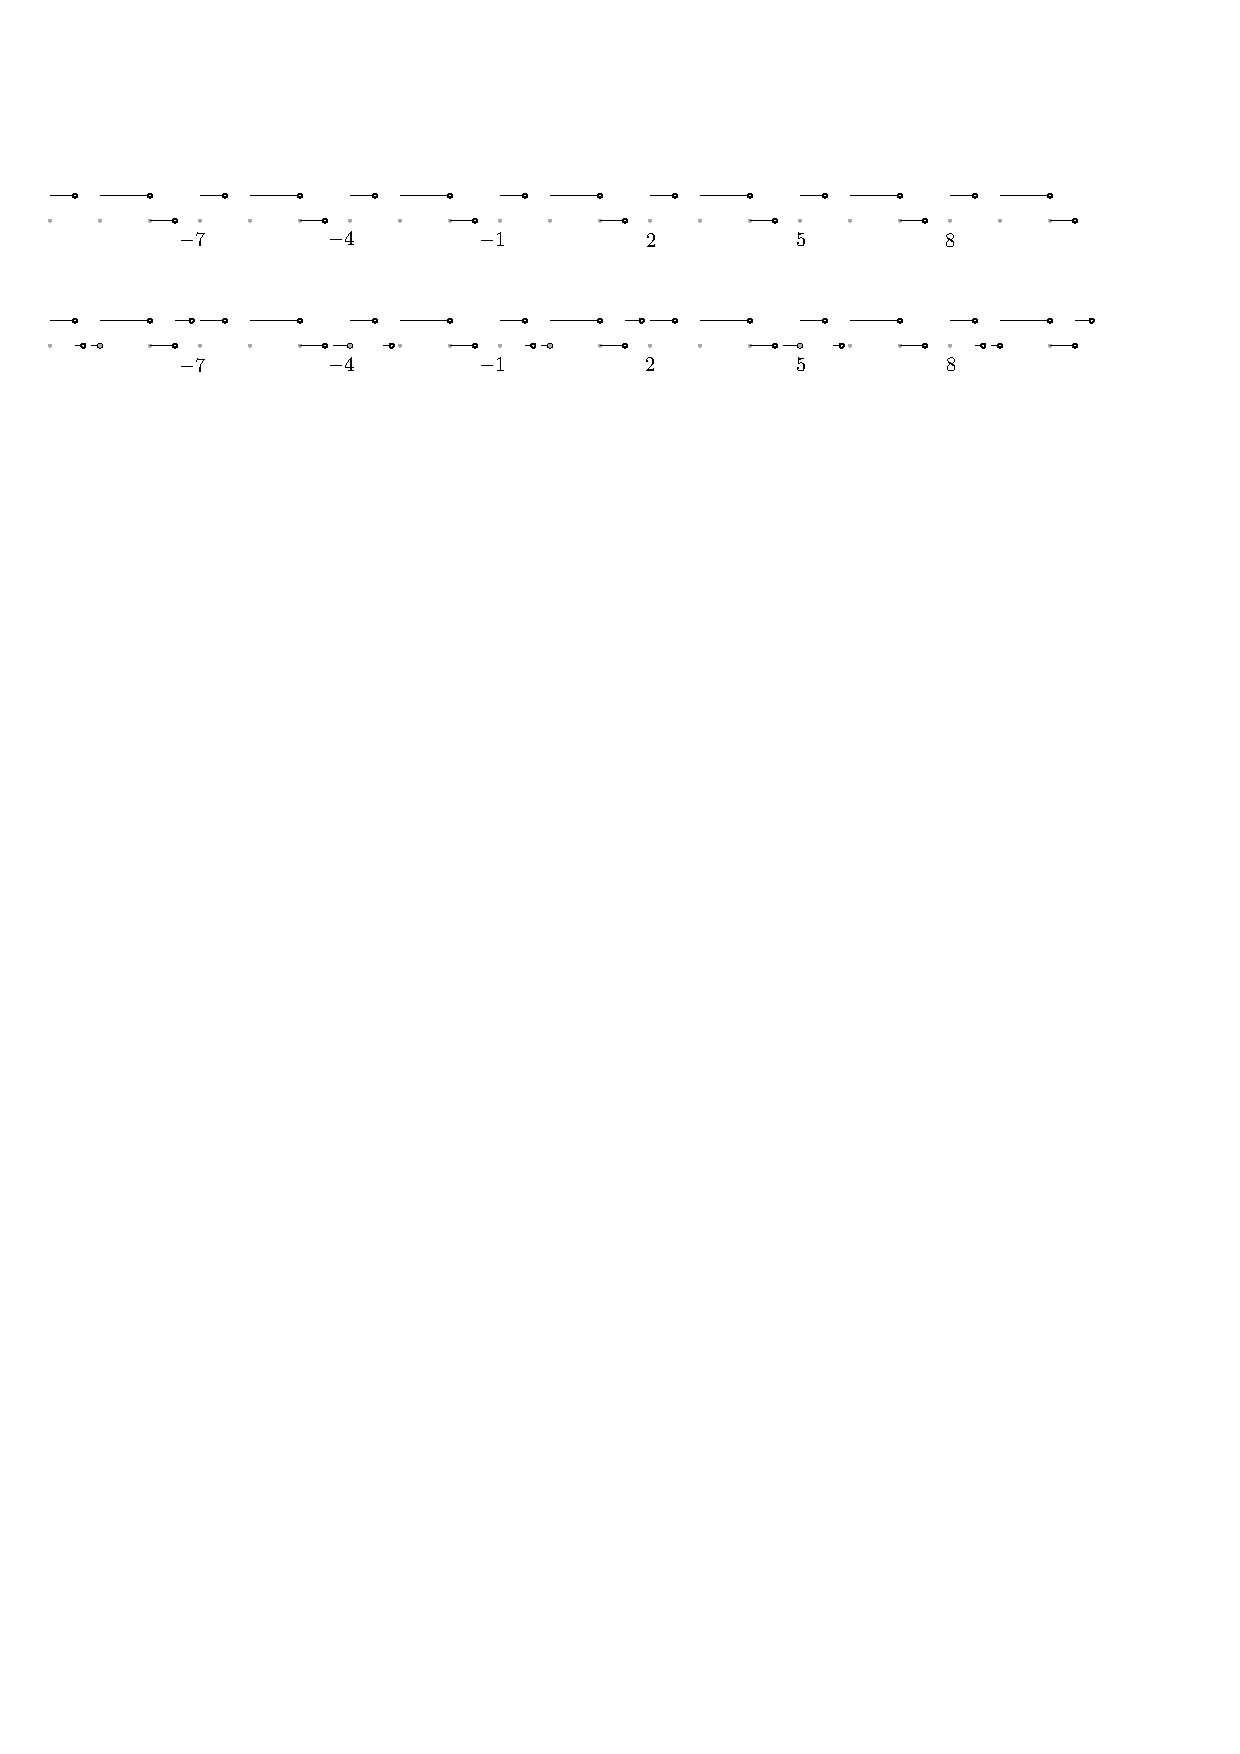
\includegraphics[scale=0.8]{Graphics/toeplitzQ2}
\caption{An illustration of the initial two steps of the construction of a quasi-Toeplitz configuration in $\Q$. }\label{fig:toeplitzQ}
\end{figure}


\section{Properties}
We are ready to prove some interesting properties of quasi-Toeplitz configurations that are instrumental in our proof of Theorem \ref{Krieger2}. 
%
The first property is that orbits of quasi-Toeplitz configurations yield minimal subsystems.
\begin{lem}\label{lem:toeplitz-minimal}
If $x\in\alf^G$ is a quasi-Toeplitz configuration with respect to a congruent \Folner sequence  $\F=\{F_n\}_{n\in\N}$, then $\closure{Gx}$ is a minimal set.
\end{lem}

\begin{proof}
By Theorem \ref{thm:minimal-synd} it is enough to show that $N(x,\{x\}^\eps)$ is syndetic for every $\eps>0$. (Recall that $N(x,A)=\{g\in G: gx\in A\}$, where $x\in X$ and $A\subseteq X$; and $B^\eps$ is an $\eps$-hull of a set $B\subseteq X$.)

Fix $\eps>0$ and take $F\subseteq G$ such that $|F|^{-1}<\eps$.
%
It suffices to prove that the set $$\{g\in G: g x_{F} = x_{F}\}$$ is syndetic. To this end, it is enough to show that  
\begin{equation}\label{eq:Cm}
C_n\subseteq \{g\in G: g x_{F} = x_{F}\}
\end{equation}
for some $n\in \N$ since $C_n$ is syndetic ($F_nC_n=G$).  Choose $N\in\N$ such that $F\subseteq F_N$. By the definition of $x$, there exists $m\geq N$ such that $x_{F_N} = x_{F_Nc}$ for every $c\in C_m$. We show that $C_m$ satisfies (\ref{eq:Cm}) (i.e., one can take $n:=m$). Take any $c\in C_m$, then indeed $F\subseteq F_N$ implies 
\[
c x_{F} = x_{Fc} =  x_{F}.\qedhere
\]
\end{proof}

\noindent
Now we show that the family of quasi-Toeplitz configurations is path-connected with respect to the Weyl pseudometric, which is a consequence of the following lemma.

\begin{lem}\label{lem:connected1}
If $G$ is a congruent monotileable group then there exists a function $\Psi\colon[0,1]\to\{0,1\}^G$ such that $\Psi(0)=0^G$, $\Psi(1)=1^G$ and for every $s,t\in[0,1],$ $\Psi(s),\Psi(t)$ are quasi-Toeplitz configurations satisfying $D^\star(\Psi(s),\Psi(t))\leq|s-t|$.
\end{lem}

\begin{proof}
Let $\F=\{F_n\}_{n\in\N}$ be a congruent \Folner sequence in $G$ with sets $\{J_n\}_{n\in\N}$ as in Definition \ref{def:congruent_monotilable} and associated \elegant sequence of centers $\{C_n\}_{n\in\N}$. Since $G$ is countable, we can enumerate its elements as $g_1, g_2, g_3,\ldots$ such that if $g_i\in F_n$ and $g_j \in F_{n+1}\setminus F_n$, then $i<j$.  Fix $t\in[0,1]$. We define $\Psi(t)= x^{(t)}\in\{0,1\}^G$ inductively. 

In the base step we put $x_0^{(t)}\defeq \star^G\in \{0,1,\star\}^G$ (by the symbol ``$\star$'' we understand an ``empty place''). In the $(n+1)$-th step we define a quasi-periodic configuration $x_{n+1}^{(t)}\in\{0,1,\star\}^G$ such the number of $1$'s in $F_{n+1}$ divided by $|F_{n+1}|$ approximates $t$ from below with accuracy $\frac{1}{|F_n|}$ (see Figure \ref{fig:path_connect_Toeplitz}). 

Assume that we have already constructed some $x_{n}^{(t)}$. 
Denote by $k_{n+1}$ the number of $\star$'s apperaing in $x_{n}^{(t)}$ over $F_{n+1}$.
We construct $x_{n+1}^{(t)}$ by substituting all (but one) 
of these $\star$'s with $0$'s and $1$'s and then copying this new pattern we obtained over $F_{n+1}$ to the whole group $G$. We proceed as follows, choose $l_{n+1}\in\{0,1,\ldots,k_{n+1}\}$ such that the number $\frac{l_{n+1}}{k_{n+1}}$ approximates $t$ from below. Then we substitute $l_{n+1}$ stars in $F_{n+1}$ with $1$'s, $k_{n+1}-l_{n+1}-1$ stars we substitute with $0$'s and one remaining star we leave without change.
%
Next we copy the pattern we defined over $F_{n+1}$ to the whole group $G$.
Finally, we  define $x^{(t)}$ as a quasi-uniform limit of the sequence  $\inbrace{x_n^{(t)}}_{n\in\N}$.

\begin{figure}
\centering
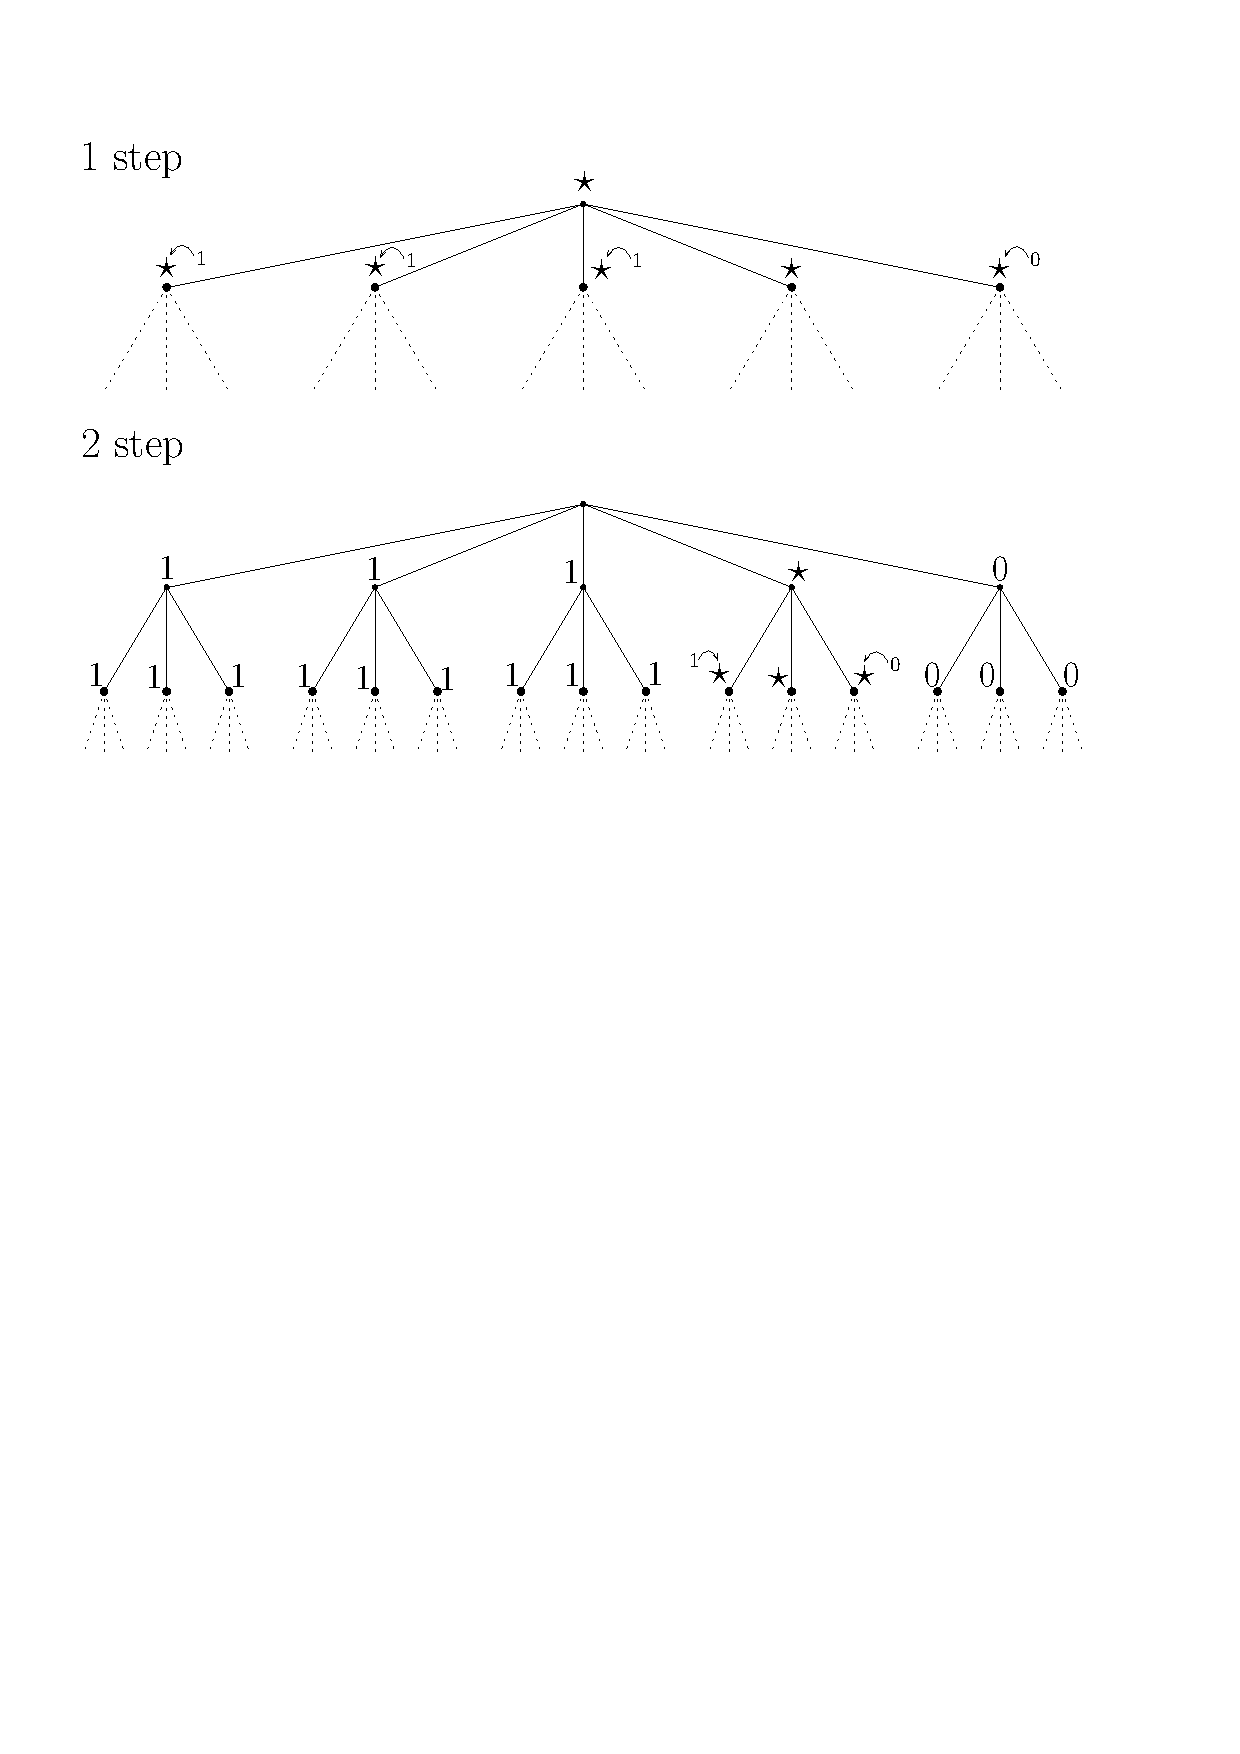
\includegraphics[scale=0.85]{Graphics/toeplitz_path_tree}
\caption{An illustration of the first two steps of the construction from the proof of Lemma \ref{lem:connected1} for $t=0.7$. (For the construction of the tree graph of $G$ see Figure \ref{fig:tree}.) Sample set $F_{1}$ consists of $5$ elements (all vertices of depth $1$). The initial state in the first step is $F_1$ filled with $\star$'s. We need to decide how many $\star$'s we replace with $1$'s and how many with $0$'s. Hence we need to find  $k=0,1,\ldots, 5$ satisfying $\frac{k}{5}< 0.7 \leq \frac{k+1}{5}$. Clearly, $k=3$. Therefore the first three $\star$'s we replace with $1$'s, the next star we leave without change, and  the remaining star we replace by zero (according to the global ordering of $G$). Next we copy this pattern using $C_1$  to the all $G$. In the second step we are interested in vertices of depth $2$. There are three $\star$'s in $F_{2}$ hence we need to choose $k=0,1,2,3$ such that $\frac{9+k}{15}< 0.7 \leq \frac{9+k+1}{15}$. Thus $k=1$, which means that the first star we replace by $1$, the next star we leave without change, and  the remaining star we replace by $0$. Then we copy this pattern using $C_2$ to the all $G$. }\label{fig:path_connect_Toeplitz}
\end{figure}



Formally, let $D_0(t)=\emptyset$ and $E_0(t)=\emptyset$. In the $(n+1)$-th step we construct sets $D_{n+1}(t)\subseteq G$ and  $E_{n+1}(t)\subseteq G$ which determine positions of $1$'s and $0$'s in $x_{n+1}^{(t)}$ respectively.
Assume that we have already defined sets $D_n(t)$ and $E_n(t)$ for some $n\in\N$. Let $f\in G$  be the position occupied by the ``star'' in $F_{n}$ after the $n$-th step of the construction, that is,
\[
\{f\}\defeq F_{n}\setminus(D_n(t)\cup E_n(t)).
\]
Then $fJ_n$ is the set of positions occupied by $\star$'s in $F_{n+1}$ after the $n$-th step of the construction. Denote $s:=|J_n|$ and let  $f_1,f_2,\ldots, f_s$ be the elements of $fJ_n$ indexed as given by the global ordering of $G$. Denote by $p$ the number of $1$'s in $F_{n+1}$ after the $n$-th step of the construction, i.e.,
 \[
 p\defeq \inmodul{D_n(t)\cap F_{n+1}}.
 \]
 Next we choose the number of $\star$'s in $F_{n+1}$ that we replace with $1$'s:
\begin{equation}\label{eq:def_q}
q\defeq\max\inbrace{\tilde q\,:\, \tilde q\in\{0,1,\ldots, s\} \,\text{ and }\, \frac{p+\tilde q}{|F_{n+1}|}< t},
\end{equation}
and define 
\begin{align*}
&D_{n+1}(t)\defeq D_n(t)\cup\inbrace{f_1,f_2,\ldots,f_q}C_{n+1},
\\
&E_{n+1}(t)\defeq E_n(t)\cup\inbrace{f_{q+2},f_{q+3},\ldots,f_s} C_{n+1}.
\end{align*}
At the end we have constructed sequences 
\[
D_0(t)\subseteq D_1(t)\subseteq D_2(t)\subseteq\ldots \quad\quad\text{ and }\quad \quad E_0(t)\subseteq E_1(t)\subseteq E_2(t)\subseteq\ldots .
\] 
Denote their unions by:
\[
D(t)\defeq \bigcup_{n\in\N}D_n(t)\quad \text{ and }\quad E(t)\defeq \bigcup_{n\in\N}E_n(t).
\]
Notice that $D(t)\cup E(t)=G$ and $D(t)\cap E(t)=\emptyset$. Then $x^{(t)}\in\{0,1\}^G$ given by 
 \begin{equation*}
x^{(t)}(g)\defeq \begin{cases} 1\quad\text{if }g\in D(t),\\
0\quad\text{if }g\in E(t)
\end{cases}
\end{equation*}
is a quasi-Toeplitz configuration. Hence the function $\Psi(t)= x^{(t)}$ satisfies the first two claims.
To justify that it is quasi-continuous (i.e., continuous with respect to $D_W$), fix $s,t\in [0,1]$ with $s<t$. Note that if $D_n(s)$ and $D_n(t)$  are as in the construction above, then $D_n(s)\subseteq D_n(t)$ for every $n\in\N$. To prove this, one has to consider the first step of the construction $N\in\N$ such that $D_N(t)\neq D_N(s)$. Next, observe that $D_N(s)\subseteq D_N(t)$. Then proceed inductively. This fact implies that
\[
D^\star\inparen{ x^{(s)}, x^{(t)}}=D^\star\inparen{\inbrace{g\in G\,:\,x^{(s)}(g)\neq x^{(t)}(g)}} = D^\star(D(t)\setminus D(s)).
\]
Now we show that $D^\star(D(t)\setminus D(s)) = t-s$. To this end, observe that Lemma \ref{ECdensity} applied to $E:=D_n(t)\cap F_n$ and $F:=F_n$ yields
\[
D^\star(D_n(t))=\frac{|D_n(t)\cap F_n|}{|F_n|}.
\]
Hence, by the construction (see (\ref{eq:def_q})) and again applying Lemma \ref{ECdensity}, one has
\begin{equation}\label{eq:Dnt_density}
D^\star(D_n(t))<t \leq D^\star(D_n(t))+\frac{1}{|F_n|} = D^\star(D'_n(t)),
\end{equation}
where $D'_n(t) := G\setminus E_n(t)$. Since 
$D_n(t)\setminus D'_n(s)\subseteq D(t)\setminus D(s)$ for every $n\in \N$ and $D_n'(s)\subseteq D_n(t)$
for $n$ large enough,
combining (\ref{eq:Dnt_density}) with Lemma \ref{lem:Dstar_properties} we obtain 
\begin{equation}\label{Dt_dens_below}
t-s - \frac{2}{|F_n|} \leq D^\star(D(t)\setminus D(s)) 
\end{equation}
for $n$ large enough. Analogously we show that $D(t)\setminus D(s) \subseteq D'_n(t)\setminus D_n(s) $ implies 
\begin{equation}\label{Dt_dens_above}
D^\star(D(t)\setminus D(s)) \leq t-s +\frac{2}{|F_n|}.
\end{equation}
Combining \eqref{Dt_dens_below}, \eqref{Dt_dens_above} and passing with $n$ to $\infty$ yields $D^\star(D(t)\setminus D(s)) = t-s$.
\end{proof}


\begin{lem}\label{lem:connected2}
Let $\alf$ be a finite alphabet and let $\F=\{F_n\}_{n\in\N}$ be a congruent \Folner sequence with associated \elegant sequence of centers $\mC=\{C_n\}_{n\in\N}$.
Then the family of quasi-Toeplitz configurations with respect to  $\F$ and $\mC$ over $\alf^G$ is $D_W$-path-connected.
\end{lem}

\begin{proof}
We can realize any finite alphabet $\alf$ as a discrete subset of $\R$, i.e., assume that $\alf\subseteq \mathbb R$.
%
Pick two quasi-Toeplitz configurations $z,z'\in \alf^G$ with respect to $\F$ and $\mC$. 
We construct a path 
\[
\{u^{(t)}\,:\,t\in[0,1]\}\subseteq \alf^G
\]
connecting $z$ with $z'$.
%
Let $\Psi\colon[0,1]\to\{0,1\}^G$ and $ x^{(t)}\in\{0,1\}^G$ for $t\in[0,1]$ be defined as in Lemma~\ref{lem:connected1} with $\F$ and $\mC$ in the construction. 
%
For $t\in[0,1]$ define $u^{(t)}\in\alf^G$ by 
\[
{u}^{(t)}(g)\defeq x^{(t)}(g){z}(g)+(1-x^{(t)}(g)) {z}'(g).
\]
Note that  $D^\star(u^{(s)},u^{(t)})\leq D^\star(x^{(s)},x^{(t)})$ and $D^\star( x^{(s)}, x^{(t)})\to 0\text{ as }s\to t.$ Now we show that $u^{(t)}$ is a quasi-Toeplitz configuration for every $t\in[0,1]$. Fix $t\in[0,1]$ and $g\in G$. We will find $N\in\N$ such that ${u}^{(t)}(gh)={u}^{(t)}(g)$ for every $h\in C_N$. Since $x^{(t)}$, $z$ and $z'$ are quasi-Toeplitz configurations with respect to $\F$, there exist $n_1,n_2,n_3\in\N$ such that $g\in\text{Per}_{C_{n_1}}(x^{(t)})$, $g\in  \text{Per}_{C_{n_2}}( z)$ and $g\in  \text{Per}_{C_{n_3}}(z')$.  Choose $N=\max\{n_1,n_2,n_3\}$. Then $C_N\subseteq C_{n_i}$ for $i=1,2,3$.
Therefore for every $h\in C$ one has 
\[
{u}^{(t)}(gh)=x^{(t)}(gh) {z}(gh) +(1-x^{(t)}(gh)) {z}'(gh)=x^{(t)}(g){z}(g)+(1-x^{(t)}(g)) {z}'(g)={u}^{(t)}(g). \qedhere
\]
\end{proof}

\noindent 
We conclude this section with an interesting, auxiliary result on regular quasi-Toeplitz configurations.
%
Let us start by a definition.
\begin{defn}
We call a quasi-Toeplitz configuration $x\in \alf^G$ {\bf regular}
if there exists a congruent sequence $\{F_n\}_{n\in\N}$ with an \elegant sequence of centers $\{C_n\}_{n\in\N}$ such that
\[
\sup_{n\in\N} D^\star\big(\text{Per}_{C_n}( x)\big)=1.
\]
\end{defn}
\begin{lem}\label{sss}
Every regular quasi-Toeplitz configuration is a quasi uniform limit of a sequence of quasi-periodic configurations.
\end{lem}

\begin{proof}
Let $x\in\alf^G$ be a regular quasi-Toeplitz configuration with a congruent sequence $\{F_n\}_{n\in\N}$ and an \elegant sequence of centers $\{C_n\}_{n\in\N}$.
Notice that if $m\leq n$, then $\text{Per}_{C_m}(x)\subseteq\text{Per}_{C_n}( x)$ for $m,n\in\N$.
Therefore 
\[
1=\sup_{n\in\N}D^\star(\text{Per}_{C_n}(x))=\lim\limits_{n\to\infty}D^\star(\text{Per}_{C_n}(x)).
\]
Define $x^{(n)}\in \alf^G$ as $x^{(n)}(fc)= x(f)$ for every $f\in F_n$ and $c\in C_n$.  
Then 
\[
\{g\in G\,:\,x^{(n)}(g)\neq x(g)\}\subseteq G\setminus \text{Per}_{C_n}( x),
\]
which implies 
\[
D^\star( x^{(n)}, x)\leq 1- D^\star(\text{Per}_{C_n}( x))\to 0 \quad \text{as}\quad n\to\infty. \qedhere
\]
\end{proof}

